\subsection{Challenge Identification}\label{challenges}

In order to effectively evaluate the task at hand the challenges involved must first be identified. With regards to this the following challenges were identified as being the most important overall aims for the project, at least in the current stage. 

\begin{itemize}
	\item What to measure?

	In order to measure air quality effectively a standard definition should be used. Research proved that there was very little consensus on the definition of air quality and so a definition which this thesis will use as the standard must be defined. The definition must also include a list of chemicals so that the appropriate hardware can be used to generate readings. This ensures that the solution is also cost effective. 

	\item Deployment considerations

	\todo[inline]{Should this be in a seperate section?}

	In the MInf Project Proposal stage it was discovered that there are certain considerations which must be made in order to effectively measure air quality. As can be seen in Figure~\ref{fig:stationarypollutantbuildup}, which shows the initial motion of a bus with an air quality sensor on the top deck, pollutants build up when the bus is stationary and only disperse after a certain amount of time which is dependent on the current weather and motion of the bus.

	\begin{figure}[H]
        \begin{center}
                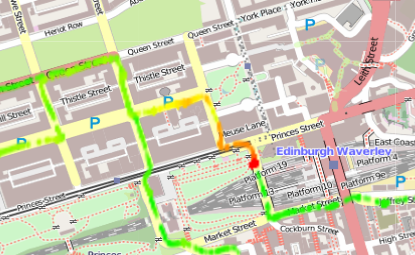
\includegraphics[scale=0.8]{./images/mpp1/StationaryPollutantBuildUp.png} 
                \caption{Example of pollutant build up in stationary situations. In this example the bus starts where the highest concentration of pollutants is found, denoted by the red, and moves in a northern direction initially.}
                \label{fig:stationarypollutantbuildup}
        \end{center}
	\end{figure}

	\todo[inline]{Should this be full width or corrected to be the width of the table?}

	It was also found that certain measurements were dependant on other factors. Temperature, for instance, was dependant on the direction of the bus due to the sensors location at the back of the bus. When the bus turned towards the south, the sunlight hit the temperature sensor directly which caused a spike in temperature readings. Humidity showed a similar response to the air pollutants. \todo{Link to data}

	With regards to this it has been determined that in order to continue with the original plan of mounting the sensors on buses, a suitable enclosure must be designed which will remove direct sunlight and build up of pollutants from the data. It may be that it is not possible to remove the pollutant build up and stops may need to be recorded so that the data can be corrected for this discrepancy, whether by adjusting the recorded values automatically, or simply removing it from the data set. 

	\item Calibration

	Each sensor is different from other models and even subtly different from other samples of the same model. In order to compensate for this calibration must be performed. In certain situations it may be sufficient to simply measure against a baseline before starting the data collection, however in others calibration may be needed periodically. 

	Projects such as the OpenSense deployment in Zurich~\cite{opensensezurich} perform periodic calibrations when the trams come within a certain distance of each other. 


	\item Data collection
	
	Data collection is the main goal of this project. The aim of this is to have a method which is both efficient, in terms of power consumption and reliability, and responsive. In order to do this there are multiple methods of uploading data which can be trialled to find that which is the most effective.

	\item Interpolating and extrapolation

	When dealing with a data set such as air quality readings where we only have sparse data measurements it is important to represent the data as clearly as possible. In order to do this a method of interpolation, and potentially extrapolation, must be employed. Three \todo{Confirm that it's 3} different models will be evaluated and compared in order to select the model which is most appropriate for generating the expected output.

\end{itemize}

